% Created by tikzDevice version 0.12 on 2019-05-31 15:23:01
% !TEX encoding = UTF-8 Unicode
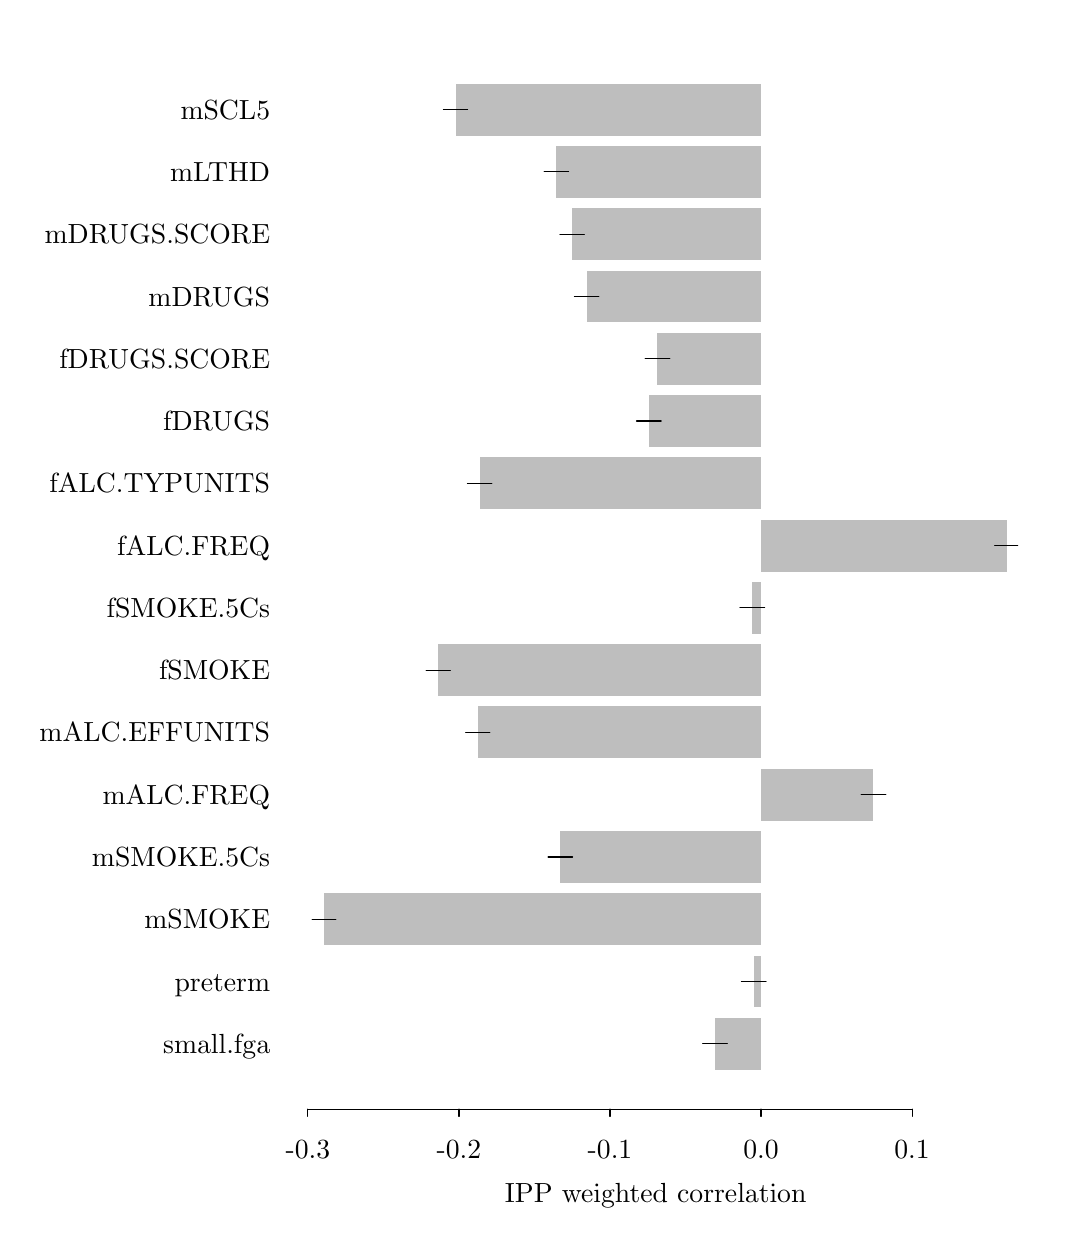
\begin{tikzpicture}[x=1pt,y=1pt]
\definecolor{fillColor}{RGB}{255,255,255}
\path[use as bounding box,fill=fillColor,fill opacity=0.00] (0,0) rectangle (369.89,426.79);
\begin{scope}
\path[clip] (  0.00,  0.00) rectangle (369.89,426.79);
\definecolor{fillColor}{RGB}{190,190,190}

\path[fill=fillColor] (265.00, 50.25) rectangle (248.35, 69.00);

\path[fill=fillColor] (265.00, 72.75) rectangle (262.38, 91.51);

\path[fill=fillColor] (265.00, 95.26) rectangle (107.09,114.01);

\path[fill=fillColor] (265.00,117.76) rectangle (192.47,136.51);

\path[fill=fillColor] (265.00,140.26) rectangle (305.62,159.01);

\path[fill=fillColor] (265.00,162.76) rectangle (162.61,181.52);

\path[fill=fillColor] (265.00,185.27) rectangle (148.37,204.02);

\path[fill=fillColor] (265.00,207.77) rectangle (261.86,226.52);

\path[fill=fillColor] (265.00,230.27) rectangle (353.84,249.02);

\path[fill=fillColor] (265.00,252.77) rectangle (163.31,271.53);

\path[fill=fillColor] (265.00,275.28) rectangle (224.46,294.03);

\path[fill=fillColor] (265.00,297.78) rectangle (227.57,316.53);

\path[fill=fillColor] (265.00,320.28) rectangle (201.99,339.03);

\path[fill=fillColor] (265.00,342.78) rectangle (196.72,361.53);

\path[fill=fillColor] (265.00,365.29) rectangle (191.05,384.04);

\path[fill=fillColor] (265.00,387.79) rectangle (154.60,406.54);
\definecolor{drawColor}{RGB}{0,0,0}

\node[text=drawColor,anchor=base,inner sep=0pt, outer sep=0pt, scale=  1.00] at (226.94,  2.40) {IPP weighted correlation};
\end{scope}
\begin{scope}
\path[clip] (  0.00,  0.00) rectangle (369.89,426.79);
\definecolor{drawColor}{RGB}{0,0,0}

\path[draw=drawColor,line width= 0.4pt,line join=round,line cap=round] (101.27, 36.00) -- (319.58, 36.00);

\path[draw=drawColor,line width= 0.4pt,line join=round,line cap=round] (101.27, 36.00) -- (101.27, 33.38);

\path[draw=drawColor,line width= 0.4pt,line join=round,line cap=round] (155.85, 36.00) -- (155.85, 33.38);

\path[draw=drawColor,line width= 0.4pt,line join=round,line cap=round] (210.43, 36.00) -- (210.43, 33.38);

\path[draw=drawColor,line width= 0.4pt,line join=round,line cap=round] (265.00, 36.00) -- (265.00, 33.38);

\path[draw=drawColor,line width= 0.4pt,line join=round,line cap=round] (319.58, 36.00) -- (319.58, 33.38);

\node[text=drawColor,anchor=base,inner sep=0pt, outer sep=0pt, scale=  1.00] at (101.27, 18.00) {-0.3};

\node[text=drawColor,anchor=base,inner sep=0pt, outer sep=0pt, scale=  1.00] at (155.85, 18.00) {-0.2};

\node[text=drawColor,anchor=base,inner sep=0pt, outer sep=0pt, scale=  1.00] at (210.43, 18.00) {-0.1};

\node[text=drawColor,anchor=base,inner sep=0pt, outer sep=0pt, scale=  1.00] at (265.00, 18.00) {0.0};

\node[text=drawColor,anchor=base,inner sep=0pt, outer sep=0pt, scale=  1.00] at (319.58, 18.00) {0.1};

\node[text=drawColor,anchor=base east,inner sep=0pt, outer sep=0pt, scale=  1.00] at ( 87.60, 56.18) {small.fga};

\node[text=drawColor,anchor=base east,inner sep=0pt, outer sep=0pt, scale=  1.00] at ( 87.60, 78.69) {preterm};

\node[text=drawColor,anchor=base east,inner sep=0pt, outer sep=0pt, scale=  1.00] at ( 87.60,101.19) {mSMOKE};

\node[text=drawColor,anchor=base east,inner sep=0pt, outer sep=0pt, scale=  1.00] at ( 87.60,123.69) {mSMOKE.5Cs};

\node[text=drawColor,anchor=base east,inner sep=0pt, outer sep=0pt, scale=  1.00] at ( 87.60,146.19) {mALC.FREQ};

\node[text=drawColor,anchor=base east,inner sep=0pt, outer sep=0pt, scale=  1.00] at ( 87.60,168.70) {mALC.EFFUNITS};

\node[text=drawColor,anchor=base east,inner sep=0pt, outer sep=0pt, scale=  1.00] at ( 87.60,191.20) {fSMOKE};

\node[text=drawColor,anchor=base east,inner sep=0pt, outer sep=0pt, scale=  1.00] at ( 87.60,213.70) {fSMOKE.5Cs};

\node[text=drawColor,anchor=base east,inner sep=0pt, outer sep=0pt, scale=  1.00] at ( 87.60,236.20) {fALC.FREQ};

\node[text=drawColor,anchor=base east,inner sep=0pt, outer sep=0pt, scale=  1.00] at ( 87.60,258.71) {fALC.TYPUNITS};

\node[text=drawColor,anchor=base east,inner sep=0pt, outer sep=0pt, scale=  1.00] at ( 87.60,281.21) {fDRUGS};

\node[text=drawColor,anchor=base east,inner sep=0pt, outer sep=0pt, scale=  1.00] at ( 87.60,303.71) {fDRUGS.SCORE};

\node[text=drawColor,anchor=base east,inner sep=0pt, outer sep=0pt, scale=  1.00] at ( 87.60,326.21) {mDRUGS};

\node[text=drawColor,anchor=base east,inner sep=0pt, outer sep=0pt, scale=  1.00] at ( 87.60,348.72) {mDRUGS.SCORE};

\node[text=drawColor,anchor=base east,inner sep=0pt, outer sep=0pt, scale=  1.00] at ( 87.60,371.22) {mLTHD};

\node[text=drawColor,anchor=base east,inner sep=0pt, outer sep=0pt, scale=  1.00] at ( 87.60,393.72) {mSCL5};
\end{scope}
\begin{scope}
\path[clip] ( 96.00, 36.00) rectangle (357.89,420.79);
\definecolor{drawColor}{RGB}{0,0,0}

\path[draw=drawColor,line width= 0.4pt,line join=round,line cap=round] (252.81, 59.63) -- (243.89, 59.63);

\path[draw=drawColor,line width= 0.4pt,line join=round,line cap=round] (266.84, 82.13) -- (257.92, 82.13);

\path[draw=drawColor,line width= 0.4pt,line join=round,line cap=round] (111.36,104.63) -- (102.82,104.63);

\path[draw=drawColor,line width= 0.4pt,line join=round,line cap=round] (196.90,127.13) -- (188.05,127.13);

\path[draw=drawColor,line width= 0.4pt,line join=round,line cap=round] (310.07,149.64) -- (301.17,149.64);

\path[draw=drawColor,line width= 0.4pt,line join=round,line cap=round] (167.00,172.14) -- (158.23,172.14);

\path[draw=drawColor,line width= 0.4pt,line join=round,line cap=round] (152.73,194.64) -- (144.01,194.64);

\path[draw=drawColor,line width= 0.4pt,line join=round,line cap=round] (266.32,217.14) -- (257.40,217.14);

\path[draw=drawColor,line width= 0.4pt,line join=round,line cap=round] (358.25,239.65) -- (349.44,239.65);

\path[draw=drawColor,line width= 0.4pt,line join=round,line cap=round] (167.69,262.15) -- (158.92,262.15);

\path[draw=drawColor,line width= 0.4pt,line join=round,line cap=round] (228.91,284.65) -- (220.01,284.65);

\path[draw=drawColor,line width= 0.4pt,line join=round,line cap=round] (232.02,307.15) -- (223.11,307.15);

\path[draw=drawColor,line width= 0.4pt,line join=round,line cap=round] (206.42,329.66) -- (197.56,329.66);

\path[draw=drawColor,line width= 0.4pt,line join=round,line cap=round] (201.14,352.16) -- (192.29,352.16);

\path[draw=drawColor,line width= 0.4pt,line join=round,line cap=round] (195.47,374.66) -- (186.63,374.66);

\path[draw=drawColor,line width= 0.4pt,line join=round,line cap=round] (158.97,397.16) -- (150.23,397.16);
\end{scope}
\end{tikzpicture}
